\documentclass{standalone}
\usepackage{tikz}
\usepackage{tikz-feynman} % Paquete para diagramas de Feynman
\usepackage{amsmath} % Para el símbolo de la llave

\begin{document}

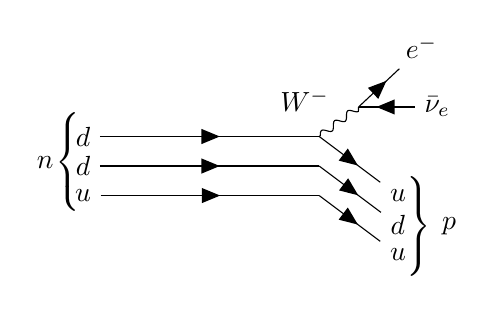
\begin{tikzpicture}
    \begin{feynman}
        % Nodos de partículas con posiciones ajustadas
        \vertex (i1) at (0,1.125) {\(d\)};
        \vertex (i2) at (0,0.75) {\(d\)};
        \vertex (i3)  at (0,{0.75/2}) {\(u\)};

        \vertex (fW) at (3.5,1.5);
        
        \vertex (f1) at (3,1.125) ;
        \vertex (f2) at (3,0.75);
        \vertex (f3) at (3,{0.75/2});

        \vertex (dw) at (3,1.125);

        \vertex (e) at (4.3,2.25) {\(e^-\)};
        \vertex (nue) at (4.5,1.5) {\(\bar{\nu}_e\)};

        \vertex (pd) at (4,0.375) {\(u\)};
        \vertex (pu1) at (4,0) {\(d\)};
        \vertex (pu2) at (4,{-0.75/2}) {\(u\)};
        
        % Nodo para la llave
        \node[left] at (-0.25,0.8){$n$};
        \node[] at (0,0.8) {\(\left\{\begin{array}{c} \\\\\\ \end{array} \right.\)};

     
        \node[] at (4.65,-0.02){$p$};
        \node[left] at (4.55,-0.02) {\(\left.\begin{array}{c} \\\\\\ \end{array} \right \}\)};

        % Diagramas de líneas
        \diagram* {
            % Líneas de quarks U
            (i1) -- [fermion] (f1),
            (i2) -- [fermion] (f2), 
            (i3) -- [fermion] (f3),  
            %Líneas bosónicas
            (dw) --[boson, edge label= $W^-$] (fW),
            % Líneas leptonicas
            (fW) -- [fermion] (e),
            (nue) -- [fermion] (fW),
            % Líneas del protón
            (dw) -- [fermion] (pd),
            (f2) -- [fermion] (pu1),
            (f3) -- [fermion] (pu2),
        };
        
    \end{feynman}
\end{tikzpicture}

\end{document}
